\section{Machine Learning : metodi e caratteristiche}
\label{ML: metodi e caratteristiche}

Lo schema logico che verrà seguito in questo capitolo prevede di approfondire inizialmente i due approcci principali al ML, ovvero l'apprendimento supervisionato(~\ref{app_sup}) e non supervisionato (~\ref{app_non_sup}), per poi presentare due metodi di apprendimento supervisionato, ovvero le $\textit{Reti Neurali}$ (~\ref{reti neurali}) e gli $\textit{Alberi Decisionali}$ (~\ref{alberi decisionali}) ed un metodo di apprendimento non supervisionato, il $\textit{Variational Autoencoders}$ (~\ref{VAEs}). Nel fare ciò verranno presentati due importanti concetti del ML, come quello di $\textit{Iperparametri}$ (~\ref{iperparametri e grid search}) ed il $\textit{Curse of dimensionality}$.

\subsection{Apprendimento supervisionato}
\label{app_sup}
In questa sezione viene portata avanti una descrizione più approfondita e formale dell'apprendimento supervisionato.\\
Come già accennato precedentemente, quando si parla di apprendimento supervisionato si hanno a disposizione sia gli input \textbf{x} che i corrispettivi target di output \textbf{y}; esisterà quindi una funzione 
\textbf{y} = f(\textbf{x}) che mette in relazione gli input con gli output. Tuttavia, come detto, tale funzione è incognita ed è quindi ciò che viene ricercato con l'algoritmo di apprendimento.
Nella pratica si cerca di approssimare la funzione agendo su una serie di parametri $\bm{\theta}$, quindi si avrà un qualcosa del tipo: \textbf{y'} = f'(\textbf{x},$\bm{\theta}$). \\

\begin{figure}[h!]
	\centering
	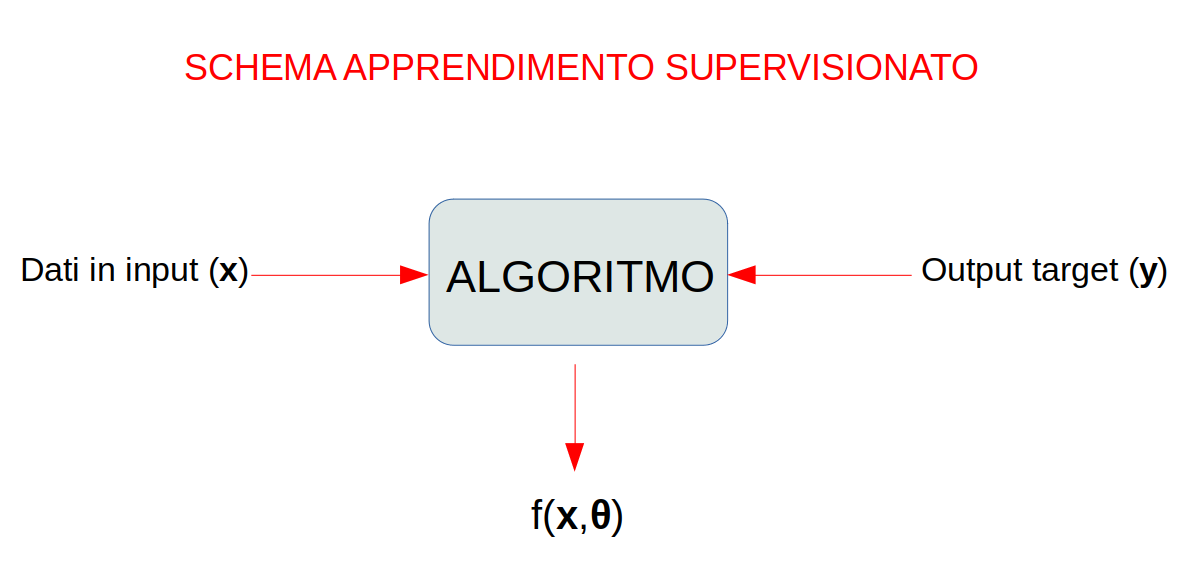
\includegraphics[width=0.85\textwidth]{figs/App_sup.png}
	\caption{si riporta uno schema intuitivo del funzionamento di un algoritmo di apprendimento supervisionato}
	\label{fig:schema_app_sup}
\end{figure}


Per ogni vettore \textbf{x} del training data set è possibile definire una particolare funzione detta "Loss function" L(\textbf{y},f(\textbf{x},$\bm{\theta}$)); a questo punto è possibile fare una media della funzione di perdita sull'intero set di dati a disposizione, ottenendo la funzione di rischio: \\
\begin{equation}
R(\bm{\theta}) = \frac{1}{N}\sum_{k=1}^{N}L(\textbf{y},f(\textbf{x},\bm{\theta}))
\end{equation}
dove N è il numero di eventi del training data set. \\
Un esempio di funzione di rischio molto diffusa è l'errore quadratico medio:
\begin{equation}
R(\bm{\theta}) = \frac{1}{N}\sum_{k=1}^{N}(\textbf{y}_k - f(\textbf{x}_k , \bm{\theta}))^2
\end{equation}
Quando si addestra un modello si vuole inoltre evitare il così detto overfitting, ovvero il fatto che il modello si è adattato troppo bene ai dati del training data set, non raggiungendo la generalità richiesta. Un modo per verificare un eventuale overfitting è quello di verificare se il modello è nettamente migliore per il data set di allenamento rispetto al data set di test. \\
Per arginare questo problema è possibile modificare la funzione di rischio, definendo la funzione di costo:
\begin{equation}
C(\bm{\theta}) = R(\bm{\theta}) + \lambda Q(\bm{\theta})
\end{equation}
con $\lambda$ parametro.
A questo punto l'obiettivo è quello di minimizzare la funzione di rischio (o di costo in caso di overfitting) e per fare ciò esistono diversi metodi, fra i quali il più comune è il metodo di discesa del gradiente.


\subsection{Discesa del gradiente}
\label{discesa del gradiente}
La discesa del gradiente è una tecnica di ottimizzazione utilizzata per minimizzare l'errore che si introduce stimando la \textbf{y'} = f'(\textbf{x},$\bm{\theta}$) rispetto alla funzione "vera" \textbf{y} = f(\textbf{x}). \\
Si consideri quindi una Loss function L(\textbf{y},f(\textbf{x},$\bm{\theta}$)) ed un vettore dei parametri $\bm{\theta}$ con i quali è possibile calcolare: \\
\begin{equation}
\textbf{G} = \frac{1}{N} \sum_{k=1}^{N} \boldsymbol{\nabla}_\theta L(\textbf{y},f(\textbf{x},\bm{\theta})) 
\end{equation} 
Una volta calcolato \textbf{G} è possibile aggiornare il vettore dei parametri $\bm{\theta}$ nel modo seguente:
\begin{equation}
\bm{\theta} - \epsilon\textbf{G} \rightarrow \bm{\theta}
\end{equation}
Qui $\epsilon$ prende il nome di passo ed ha il ruolo di calibrare di quanto debba essere modificato il vettore \bm{$\theta$} nella direzione opposta a quella del gradiente \textbf{G}.\\
Per completezza si riporta il fatto che, quando si ha un elevato campione nel training data set, si utilizza il metodo di discesa del gradiente stocastico, che è strutturato allo stesso modo di quello appena descritto ma viene limitato ad un sottoinsieme del data set di allenamento per una questione di lunghezza di calcolo.
\newpage

\subsection{Apprendimento non supervisionato}
\label{app_non_sup}

Nella sezione precedente è stata mostrata l'utilità degli algoritmi di apprendimento supervisionato, osservando che, nel caso in cui si abbiano a disposizione sia i vettori di input che i corrispettivi output target, si può ottenere un'approssimazione della relazione esistente input-output.
Tuttavia non è sempre possibile avere a disposizione gli output target e bisogna capire se è comunque possibile ottenere informazioni utili dai dati. \\
Come già accennato nelle prime pagine di questa trattazione quando non si hanno a disposizione gli output target si possono applicare tecniche di apprendimento non supervisionato, dove l'obiettivo è quello di trovare eventuali partizioni degli input (Clustering). \\
Si consideri la figura ~\ref{Unsup} dove sono riportate tre diverse configurazioni possibili nel caso di input bidimensionali: è evidente che nel caso a) sia possibile la separazione in due sotto gruppo e nel caso b) in un unico sotto gruppo, mentre nel caso c) sembrerebbe non si possano stabilire graficamente eventuali separazioni.

\begin{figure}[h!]
	\centering
	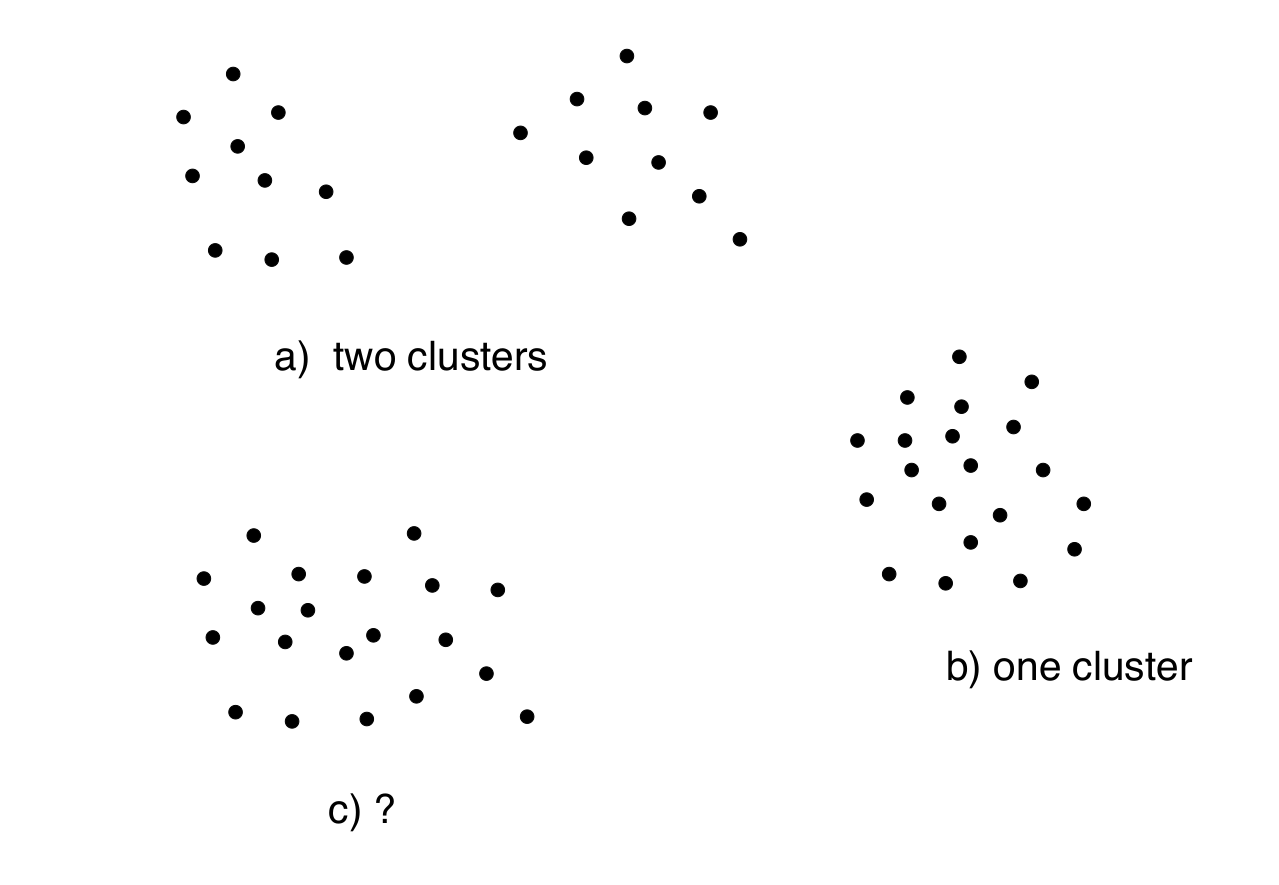
\includegraphics[width=0.85\textwidth]{figs/Unsup_learning.png}
	\caption{vettori di input in uno spazio bidimensionale in tre situazioni differenti. L'immagine è presa da \cite{IntroML}}
	\label{Unsup}
\end{figure}

Quindi un algoritmo di clustering si occupa della suddivisione del set di input $\Sigma$ in un numero N di sottogruppi $\Sigma_1$,...,$\Sigma_n$, detti appunto cluster; si noti che lo stesso numero N non viene stabilito a priori e fornito all'algoritmo, ma viene anch'esso ricavato a partire dai dati. Una volta fatto sarà possibile implementare un classificatore per collegare nuovi vettori di input con i cluster precedentemente individuati.\\
Inoltre, aumentando il livello di complessità, è possibile trovare eventuali gerarchie di partizionamento, ovvero cluster di cluster.

\newpage

\subsection{Metodo di clustering basato sulla distanza euclidea}
\label{metodo distanza euclidea}
Gli algoritmi di apprendimento non supervisionato sfruttano una qualche misura di similarità per separare i pattern (gli input) nei vari cluster. Una possibilità è quella di utilizzare la semplice distanza euclidea per poter separare lo spazio n-dimensionale dei pattern in delle sotto-aree, che sono appunto i cluster. \\
Per fare ciò viene implementato un metodo iterativo, basato sulla definizione di alcuni punti particolari nello spazio dei pattern, detti "cluster seekers" (letteralmente "cercatori di cluster"). \\
Si definiscono M punti nello spazio n-dimensionale $\textbf{C}_\textbf{1},...,\textbf{C}_\textbf{M}$ e l'obiettivo è quello di fare in modo che ogni punto si muova verso il centro di ogni singolo cluster, in modo che ogni cluster abbia al suo centro uno di questi cluster seekers. \\
Come è già stato spiegato precedentemente, l'algoritmo non conosce a prescindere il numero di cluster ma riesce a ricavarlo dai pattern stessi; per questa ragione il numero di cluster seekers M è inizialmente casuale ed esiste un procedura per ottimizzarlo, che verrà illustrata in seguito. \\
I pattern del training data set $\Sigma$ vengono presentati all'algoritmo uno alla volta: per ognuno di essi ($\textbf{x}_\textbf{i}$) si cerca il cluster seekers più vicino ($\textbf{C}_\textbf{k}$) e lo si sposta verso $\textbf{x}_\textbf{i}$ nel seguente modo:
\begin{equation}
\textbf{C}_\textbf{k} + \alpha_k(\textbf{x}_\textbf{i} - \textbf{C}_\textbf{k}) \rightarrow \textbf{C}_\textbf{k}
\end{equation}
dove $\alpha_k$ è un parametro di apprendimento che determina di quanto il cluster seeker k-esimo si muove verso il punto $\textbf{x}_\textbf{i}$. \\
A questo punto è utile fare in modo che più il cluster seeker è soggetto a spostamenti minore diventa l'entità dello spostamento. Per fare ciò si definisce una massa $m_k$ e le si assegna un valore pari al numero di volte in cui $\textbf{C}_\textbf{k}$ è stato soggetto a spostamenti (quindi anche il valore della massa verrà aggiornato di volta in volta); dopodiché si assegna ad $\alpha_k$ il seguente valore
\begin{equation}
\alpha_k = \frac{1}{1 + m_k}
\end{equation} 
e, dato che ad ogni iterazione che coinvolge $\textbf{C}_\textbf{k}$ il valore di $m_k$ aumenta di una unità, il parametro di apprendimento $\alpha_k$ diminuisce di volta in volta. \\
Il risultato di questo aggiustamento è che il cluster seeker si trova sempre nel punto che rappresenta la media dei punti del cluster. \\
Una volta che sono stati presentati tutti i pattern del training data set all'algoritmo, i vari cluster seeker saranno conversi ai "centri di massa" dei cluster e la classificazione (cioè la delimitazione dei cluster nello spazio n-dimensionale) può essere fatta con una partizione dello spazio di Voronoi, di cui si riporta la seguente definizione:
\begin{quotation} \small
	\textit{In ogni insieme (topologicamente) discreto S di punti in uno spazio euclideo e per quasi ogni punto x, c'è un punto in S che è il più vicino a x. Il "quasi" è una precisazione necessaria dato che alcuni punti x possono essere equidistanti da 2 o più punti di S.
		Se S contiene solo due punti, a e b, allora il luogo geometrico dei punti equidistanti da a e b è un iperpiano, ovvero un sottospazio affine di codimensione 1. Tale iperpiano sarà il confine tra l'insieme di tutti punti più vicini ad a che a b e l'insieme di tutti i punti più vicini a b che ad a. È l'asse del segmento ab.
		In generale, l'insieme dei punti più vicini a un punto c $\in$ S che ad ogni altro punto di S è la parte interna di un politopo (eventualmente privo di bordi) detto dominio di Dirichlet o cella di Voronoi di c. L'insieme di tali politopi è una tassellatura dell'intero spazio e viene detta tassellatura di Voronoi corrispondente all'insieme S. Se la dimensione dello spazio è solo 2, è facile rappresentare graficamente le tassellazioni di Voronoi; è a questo caso che si riferisce solitamente l'accezione diagramma di Voronoi. \\
		(Wikipedia, Diagramma di Voronoi.)} 
\end{quotation}

Un esempio didattico del risultato di questa partizione è riportato in figura ~\ref{Voronoi}.
\begin{figure}[h!]
	\centering
	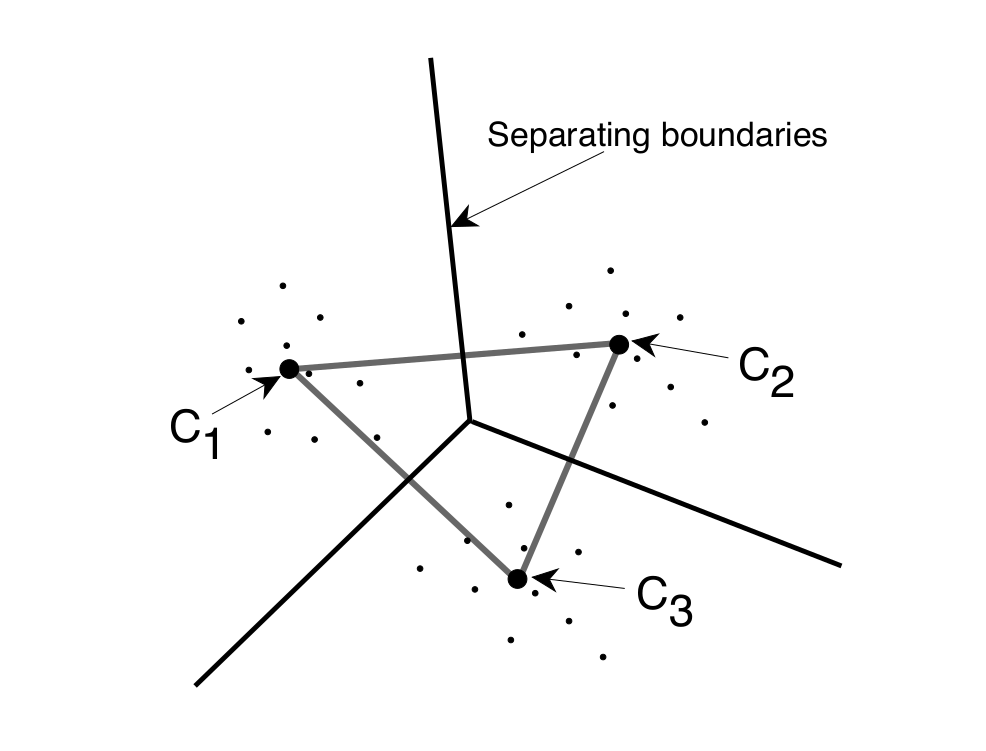
\includegraphics[width=0.70\textwidth]{figs/Voronoi.png}
	\caption{Si riporta un esempio di partizione dello spazio (bi-dimensionale) di Voronoi in tre sotto regioni . L'immagine è presa da \cite{IntroML}}
	\label{Voronoi}
\end{figure}

Si è accennato qualche riga fa che il numero di cluster seeker è inizialmente scelto in maniera casuale, per poi essere ottimizzato; per il processo di ottimizzazione si utilizza la varianza dei pattern $\{\textbf{x}_\textbf{i}\}$ per ogni cluster:
\begin{equation}
\sigma^2 = \frac{1}{L}\sum_{i=1}^{L} (\textbf{x}_\textbf{i} - \bm{\mu})^2
\end{equation}
dove L è il numero di pattern nel cluster e $\bm{\mu}$ ne è la media:
\begin{equation}
\bm{\mu} = \frac{1}{L}\sum_{i=1}^{L} \textbf{x}_\textbf{i}
\end{equation}
A questo punto, se la distanza $d_{ij}$ fra due cluster seeker $\textbf{C}_\textbf{i}$ e $\textbf{C}_\textbf{j}$ è minore di un determinato valore $\epsilon$, allora si sostituiscono i due cluster seeker con uno nuovo posto nel loro centro di massa (tenendo conto delle due masse $m_i$ e $m_j$); dall'altro lato, se vi è un cluster per il quale la varianza $\sigma^2$ è più grande di un valore $\delta$, si aggiunge un nuovo cluster seeker vicino a quello già esistente e si eguagliano entrambe le loro masse a zero.\\
Come osservazione finale bisogna dire che nei metodi che si basano sul concetto di distanza è importante ri-scalare i valori delle componenti dei pattern (in linea di principio si possono avere componenti diverse con ordini di grandezza di molto differenti) in modo da evitare che alcune componenti pesino più di altre. \\ 

\newpage

\subsection{Iperparametri e Grid Search}
\label{iperparametri e grid search}

Prima di parlare del Grid Search è necessario introdurre il concetto di \textbf{iperparametro}. Come detto nelle sezioni precedenti, un modello di apprendimento è caratterizzato da una serie di parametri che vengono modificati in maniera iterativa in modo da minimizzare la Loss function e, come noto, tale processo avviene attraverso un continuo confronto con il training data set. Quando si parla di iperparametri si intende invece una serie di parametri che caratterizzano il modello implementato che non sono modificati nel processo di addestramento con il training data set ma vengono prestabiliti dall'utente. \\
Chiaramente al variare degli iperparametri cambia anche la qualità del processo di apprendimento del modello e quindi anch'essi devono essere sottoposti ad un processo di ottimizzazione. A questo punto entra in gioco il metodo del Grid Search che è appunto un metodo di ottimizzazione degli iperparametri. \\
Il Grid Search è piuttosto semplice sia da comprendere concettualmente sia da implementare nella pratica; fa parte dei così detti "Brute-Force Search", cioè di quei metodi che si basano sulla sistematica verifica di tutte le possibili soluzioni ad un problema per poi considerare la migliore. Per esempio si consideri il problema di dover cercare i divisori di un numero n: un approccio "Brute-Force" prevedrebbe di considerare tutti i numeri minori di n e verificare quelli per i quali la divisione non dà resto. Questo esempio permette anche di mettere in evidenza il limite principale di tale tipologia di approccio: il numero di possibilità da esplorare può aumentare molto velocemente, soprattutto se si considera un processo multivariato. \\
Tornando ora nello specifico al Grid Search, si consideri un modello caratterizzato da un numero k di iperparametri. Si può definire, in analogia a ciò che è stato fatto con i parametri, un vettore le cui componenti sono appunto gli iperparametri: 
\begin{equation}
\bm{\mu} = (\mu_1,...,\mu_k)
\end{equation}
Tale vettore apparterrà ovviamente ad uno spazio k-dimensionale, sul quale può essere costruita una griglia i cui nodi corrispondono a particolari combinazioni degli iperparametri. \\
A questo punto si può avviare l'apprendimento del modello per ogni particolare configurazione degli iperparametri ed ottenere un valore per la Loss function. Si arriva allora ad avere una valore della Loss per ogni nodo della griglia e quindi basta considerare quello per il quale la Loss è minore, ottenendo la miglior configurazione degli iperparametri. \\
In Figura ~\ref{fig:Grid Search} nella pagina seguente è riportato per chiarezza un esempio visivo dell'esito di un processo di ottimizzazione degli iperparametri attraverso il metodo Grid Search.

\begin{figure}[h!]
	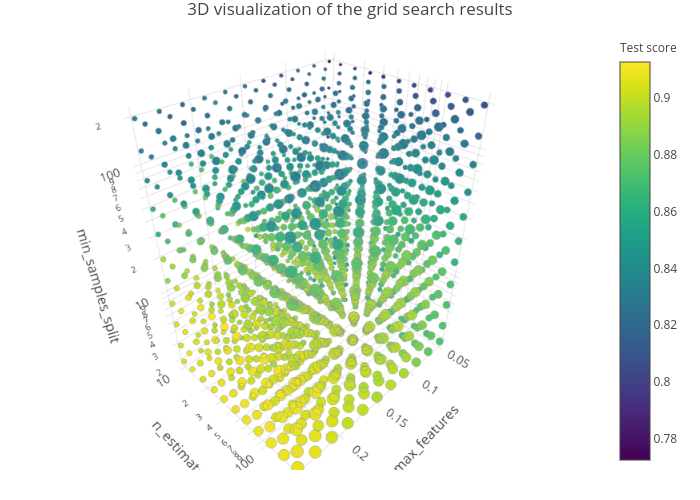
\includegraphics[width=\linewidth]{figs/Grid_immagine.png}
	\caption{la figura illustra visivamente l'esito di un processo di ottimizzazione degli iperparametri attraverso il metodo Grid Search (~\cite{knuthwebsite})}
	\label{fig:Grid Search}
\end{figure}
\newpage 

Come accennato precedentemente, man mano che aumenta la complessità del modello è molto probabile che aumenti il numero degli iperparametri e quindi la dimensionalità dello spazio introdotto precedentemente; ciò implica l'aumento considerevole del numero di configurazioni degli iperparametri da esplorare attraverso il Grid Search e quindi il tempo necessario per concludere l'ottimizzazione.\\
E' possibile ovviare parzialmente a questo problema attraverso il Random Grid Search (RGS), dove non sono considerati tutti i nodi della griglia, ma solo una loro parte selezionata in maniera casuale secondo una particolare distribuzione (ciò permette anche di tener conto di conoscenze pregresse). \\

\newpage

\subsection{Reti Neurali}
\label{reti neurali}
Le reti neurali sono probabilmente il metodo di apprendimento supervisionato più conosciuto ed utilizzato nel campo dell'analisi dati. \\
La struttura di una rete neurale prevede la presenza di unità fondamentali, dette neuroni, che sono organizzate in strati e legate fra di loro mediante delle connessioni (sinapsi), ciascuna delle quali è caratterizzata da un peso. Sono proprio questi pesi a giocare un ruolo fondamentale nel processo di apprendimento della rete perché sono loro i parametri soggetti a modifica.\\
Il nome rete neurale (artificiale) deriva dal fatto che la loro struttura è inspirata dalle corrispondenti strutture biologiche (seppur di molto semplificata). \\
In una rete neurale è sempre presente uno strato di input ed uno di output, mentre il numero di livelli nascosti può variare a seconda della complessità della rete; In figura ~\ref{fig:schemaNN} è riportato un esempio di rete neurale con un singolo strato interno nascosto.
\begin{figure}[h!]
	\centering
	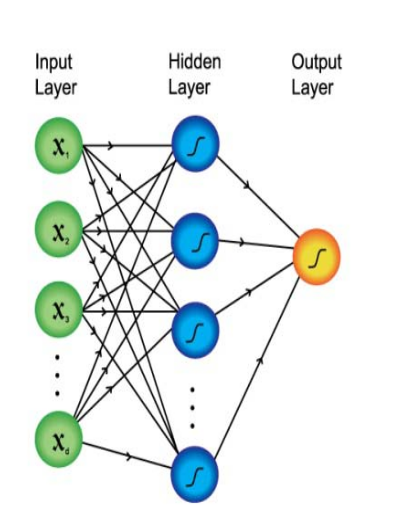
\includegraphics[width=0.50\textwidth]{figs/schemaNN.png}
	\caption{si riporta un esempio grafico di rete neurale formata da un unico strato nascosto. L'immagine è presa da \cite{Metodi_multivariati}.}
	\label{fig:schemaNN}
\end{figure}
\\
Si può passare ora a presentare il modello del singolo neurone per capire com'è strutturato e quale compito svolge.
Gli elementi che caratterizzano il singolo neurone sono:
\begin{enumerate}
	\item Una serie di connessioni in ingresso (ciascuna caratterizzata da un proprio peso);
	\item Un sommatore che ha il compito di svolgere la somma pesata degli input, utilizzando i pesi caratteristici delle connessioni;
	\item Un output e la relativa funzione di attivazione, che viene usata per limitarne l'ampiezza (tipicamente ad intervalli [0,1] o [-1,1]);
	\item Un valore di soglia che viene usato per aumentare o diminuire il valore ottenuto dalla somma pesata.
\end{enumerate}
Si riporta in figura ~\ref{schema_neurone} lo schema grafico di un singolo neurone (k), dove $\textbf{x} = (x_1 ,..., x_m)$ è il vettore degli input input, $\textbf{w}_k = (w_{k1} ,..., w_{km})$ è il vettore dei pesi, $\phi$(x) è la funzione di attivazione, $b_k$ è il valore di soglia e $y_k$ è l'output.
\begin{figure}[h!]
	\centering
	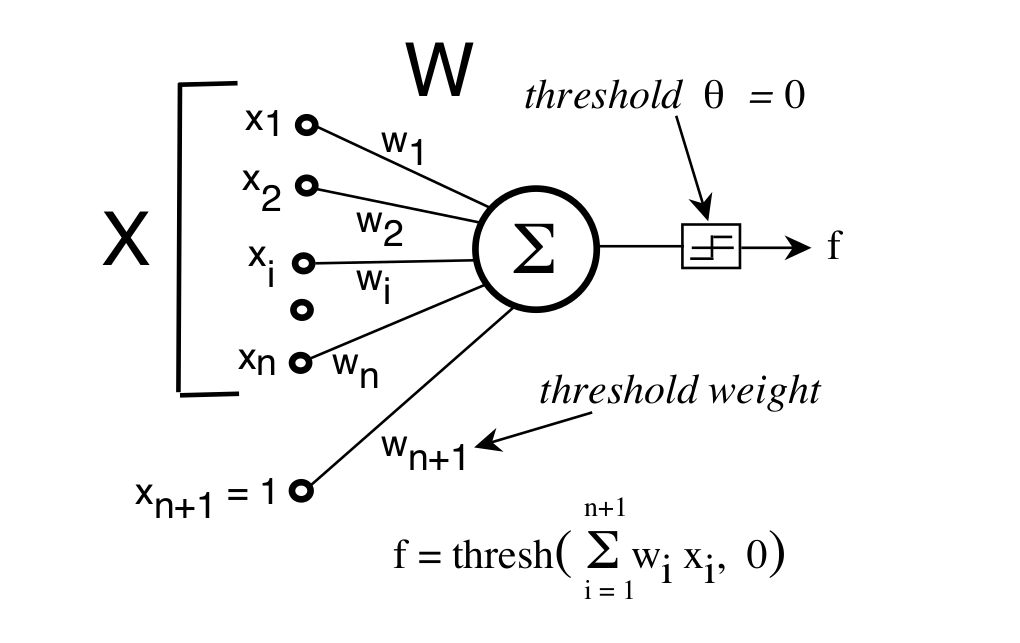
\includegraphics[width=0.70\textwidth]{figs/schema_neurone.png}
	\caption{Illustrazione della struttura di un neurone (~\cite{Intro_retiN}).}
	\label{schema_neurone}	
\end{figure} \\
Quindi il neurone opera la seguente somma pesata:
\begin{equation}
s_k = \textbf{x}\bullet\textbf{w}_\textbf{k} = \sum_{i=1}^{m}x_iw_{ki}
\label{sk}
\end{equation}
e si ottiene l'output attraverso la funzione di attivazione: 
\begin{equation}
y_k = \phi(s_k + b_k)
\end{equation}
Risulta utile spendere qualche parola in più sul tipo di funzione di attivazione più utilizzata, ovvero la funzione sigmoide:
\begin{equation}
sig(x) = \frac{1}{1 + e^{-{\alpha}x}}
\end{equation} 
dove $\alpha$ è un parametro che permette di regolare la pendenza della curva, come si evince dalla figura ~\ref{sigmoide}
\begin{figure}[h!]
	\centering
	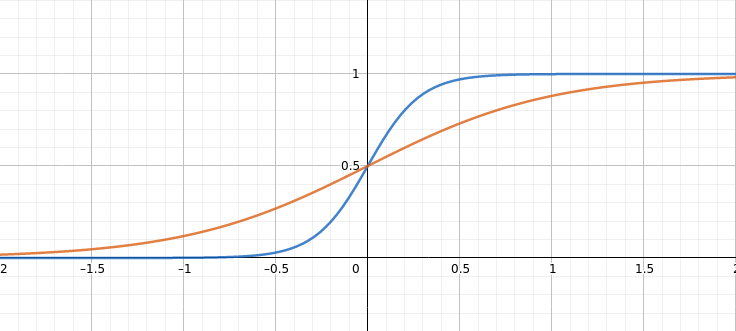
\includegraphics[width=0.75\textwidth]{figs/sigmoide.png}
	\caption{Si riportano due sigmoidi, dove per quella in rosso si ha $\alpha$=2 e per quella in blu $\alpha$=7.}
	\label{sigmoide}
\end{figure}
\newpage
Un singolo neurone è l'ingrediente fondamentale di una rete neurale e nella gran parte dei casi non è in grado di svolgere da solo nessun compito interessante ma deve sempre essere inserito in una rete. Tuttavia esiste una caso particolare nel quale un singolo neurone può portare a termine un compito di classificazione; affinché ciò sia possibile è necessario che i vettori evento siano riconducibili a due sole categorie e che il loro spazio possa essere separato (in relazione alle due categorie) da un singolo iper-piano. In questo caso esiste un teorema di convergenza che garantisce appunto la convergenza dei pesi nel processo di addestramento.

A questo punto è possibile passare ad un livello di complessità superiore, osservando in che modo possono essere organizzati i neuroni per formare la rete neurale; si distinguono due tipologie di reti:
\begin{enumerate}
	\item Reti feedforward con uno o più strati: in questo caso il segnale si propaga dai nodi di input verso quelli di output, senza connessioni fra i neuroni di uno stesso strato;
	\item Reti feedback: sono reti cicliche dove il segnale si propaga anche fra i neuroni di uno stesso strato.
\end{enumerate}
Bisogna chiedersi ora in che modo apprende il singolo neurone. Una delle possibilità (nel caso in cui sia noto l'output target) è l'apprendimento con correzione di errore, che viene presentato velocemente nel seguito.
Si consideri un singolo neurone che ha in ingresso una serie di input $(x_1,...,x_n)$ e quindi produce un valore di output $y$ attraverso la somma pesata già introdotta precedentemente; tale valore può quindi essere confrontata con il risultato atteso $R$, ottenendo così un errore $err = R - y$; si può quindi definire la funzione di costo
\begin{equation}
E = \frac{1}{2}err^2
\end{equation}
sulla quale si applicherà il metodo di discesa del gradiente già discusso nel paragrafo $2.1$ per ottimizzare i parametri.\\
Una volta capito in che modo avviene l'addestramento di un singolo neurone, è possibile trattare le diverse funzioni che può svolgere una rete neurale:
\begin{enumerate}
	\item L'associazione, a sua volta divisibile in autoassociazione ed eteroassociazione. Nel primo caso vengono presentati alla rete neurale una serie di vettori evento nella fase di training per poi verificare se uno di questi vettori, ripresentato parzialmente, viene nuovamente riconosciuto dalla rete e completato (tale funzione ben si presta ad essere ottenuta a seguito di un processo di apprendimento non supervisionato); nel secondo caso si utilizza un vettore non ancora noto alla rete neurale come richiamo di una già processato;
	\item Il riconoscimento consiste nell'associazione da parte della rete di un vettore evento ad una delle varie categorie possibili. Tale obiettivo può essere ottenuto a seguito di una fase di addestramento dove vengono forniti alla rete sia i vettori in input che le categorie alle quali questi appartengono (si tratta chiaramente di un processo di apprendimento non supervisionato). Si ipotizzi di avere a disposizione dei vettori evento con un numero n di componenti (i dati) e, chiaramente, possono essere pensati come dei punti in uno spazio n-dimensionale; questo spazio potrà essere allora diviso in delle regioni che corrispondono alle varie categorie di cui si è parlato precedentemente ed i confini di queste zone si ottengono a seguito del processo di addestramento;
	\item L'approssimazione di funzioni, dove si hanno a disposizione gli input $\textbf{x}_\textbf{i}$ ed i corrispettivi output $\textbf{y}_\textbf{i}$. Quello che si cerca di fare è approssimare al meglio la funzione $\textbf{y} = f(\textbf{x})$ vera con una $g(\textbf{x})$, tale per cui la distanza euclidea è inferiore ad un valore prefissato positivo (piccolo) $\epsilon$:
	\begin{equation}
	\Vert g(\textbf{x}) - f(\textbf{x}) \Vert < \epsilon
	\end{equation}
\end{enumerate}

Arrivati a questo punto è possibile esporre la trattazione su come una rete neurale viene addestrata. Precedentemente si è introdotta la struttura di una rete neurale, specificando le differenze fra lo strato di input, quello di output e gli strati nascosti. Ogni singolo neurone nel suo processo di addestramento deve aggiornare i suoi pesi, in modo che l'output della rete neurale sia simile a quello atteso.\\
Uno dei metodi migliori per addestrare la rete neurale è l'algoritmo di back-propagation. \\
Una rete neurale è caratterizzata da due tipologie di segnale: da un lato vi è un segnale di funzione che si propaga dallo strato di input verso quello di output e, dall'altro, vi è un segnale di errore che ha origine nello strato di output e si propaga verso quello di input. E' il segnale di errore a giocare un ruolo fondamentale nel processo di apprendimento tramite ottimizzazione dei pesi che caratterizzano la rete neurale. \\
Addentrandosi nell'algoritmo di back-propagation bisogna fare una distinzione fra il modo in cui esso viene applicato allo strato di output ed il modo in cui viene applicato agli strati nascosti:
\begin{enumerate}
	\item Neurone nello strato di output.\\
	Si consideri uno strato di output con un numero n di neuroni e ci si focalizzi sul k-esimo. In un certo momento del processo di apprendimento, alla rete neurale si starà presentando il j-esimo elemento del training data set, quindi per il neurone k si otterrà il seguente segnale di errore:
	\begin{equation}
	err_k^{(j)} = R_k^{(j)} - y_k^{(j)}
	\end{equation}
	dove con la lettera y si intende il valore ottenuto in output dal neurone e con R il valore atteso. \\
	L'errore totale dello strato di output per il vettore evento j-esimo viene definito nel seguente modo:
	\begin{equation}
	E^{(j)} = \frac{1}{2} \sum_{k=1}^{n} (err_k^{(j)})^2
	\end{equation}
	Se poi N è il numero totale di elementi del training data set, allora la funzione di costo può essere definita nel seguente modo:
	\begin{equation}
	E_{tot} = \frac{1}{N}\sum_{j=1}^{N} E^{(j)}
	\end{equation}
	e l'obiettivo è quello di minimizzare tale funzione di costo. Per fare ciò si procede aggiustando i pesi a seguito della presentazione di ogni singolo vettore evento.
	Si utilizza il metodo di discesa del gradiente, procedendo nel seguente modo: \\
	il gradiente è dato da
	\begin{equation}
	\frac{\partial E^{(j)} }{\partial w_{ki}^{(j)}}
	\end{equation}
	e gli aggiornamenti del peso vengono applicati nel verso opposto del gradiente, ovvero
	\begin{equation}
	\Delta w_{ki}^{(j)} = -\mu \frac{\partial E^{(j)} }{\partial w_{ki}^{(j)}}
	\end{equation}
	con $\mu$ fattore di apprendimento.
	Manca a questo punto il calcolo esplicito del gradiente, che può essere eseguito con la regola della catena 
	\begin{equation}
	\frac{\partial E^{(j)} }{\partial w_{ki}^{(j)}} = \frac{\partial E^{(j)}}{\partial err_k^{(j)}}
	\frac{\partial err_k^{(j)}}{\partial y_k^{(j)}}
	\frac{\partial y_k^{(j)}}{\partial S_k^{(j)}}
	\frac{\partial S_k^{(j)}}{\partial w_{ki}^{(j)}}
	\end{equation}
	dove $S_k^{(j)} = s_k^{(j)} + b_k^{(j)} $ (si faccia riferimento all'equazione \eqref{sk}). \\
	Una volta calcolate le quattro derivate si ottiene:
	\begin{equation}
	\frac{\partial E^{(j)} }{\partial w_{ki}^{(j)}} =
	-err_k^{(j)}\phi'(S_k^{(j)})y_i^{(j)}
	\end{equation}
	e quindi:
	\begin{equation}
	\Delta w_{ki}^{(j)} = err_k^{(j)}\phi'(S_k^{(j)})y_i^{(j)} \mu
	\end{equation}
	
	\item Neurone in uno strato nascosto \\
	In questo caso l'output del neurone non ha un diretto valore con il quale può essere confrontato, quindi il segnale di errore deve essere determinato a partire dai segnali di errore di tutti i neuroni dello strato successivo, da cui il nome di back-propagation proprio perché il segnale di errore prosegue all'indietro dall'output verso l'input.
\end{enumerate}
Come ultima considerazione sulle reti neurali bisogna sottolineare che il coefficiente di apprendimento deve essere scelto in maniera accurata, infatti se fosse troppo piccolo si avrebbe una convergenza estremamente lenta e, viceversa, un valore troppo grande porterebbe ad una instabilità con comportamento oscillatorio.

\newpage

\subsection{Alberi Decisionali}
\label{alberi decisionali}

Gli alberi decisionali sono, al pari delle reti neurali, un metodo ML di apprendimento supervisionato e  la loro caratteristica fondamentale è il presentarsi in maniera particolarmente intuitiva perché è possibile avere una semplice rappresentazione grafica del meccanismo del loro funzionamento. \\
Gli alberi decisionali rappresentano un mezzo estremamente interessante per le operazioni di classificazione (sia per output continui che discreti) ed operano attraverso una serie di test sugli attributi degli input (con il termine attributo si intende una componente del vettore di input ). \\ 
Come primo passo è utile discutere come è strutturato un albero decisionale, introducendo alcune notazioni (come ausilio alla trattazione si riporta in figura ~\ref{schemaDT} un esempio di albero decisionale molto semplice).\\
\begin{figure} [h!]
	\centering
	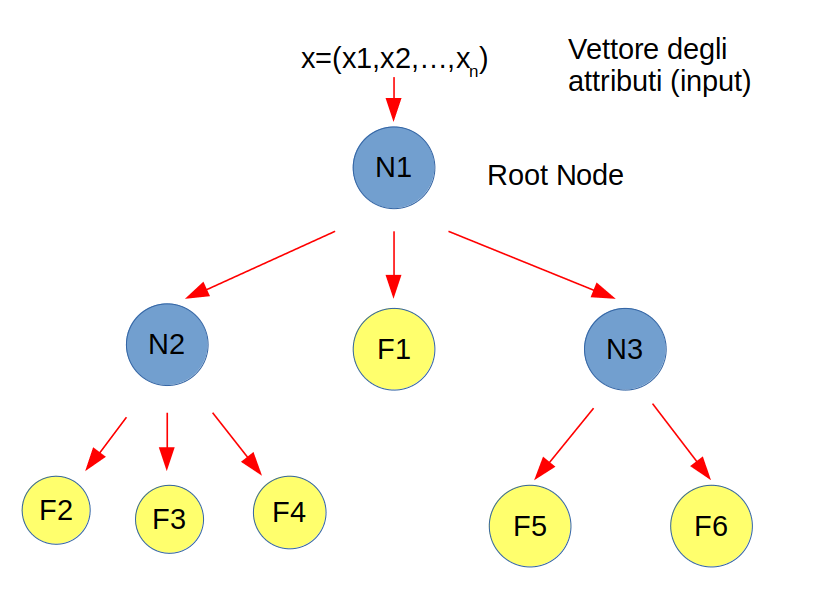
\includegraphics[width=0.70\textwidth]{figs/schemaDT.png}
	\caption{esempio di come è strutturato un albero decisionale}
	\label{schemaDT}
\end{figure}
Gli elementi che caratterizzano un albero decisionale sono:
\begin{itemize}
	\item Nodo. \\
	I nodi sono riportati in figura ~\ref{schemaDT} come dei cerchi colorati in azzurro e contrassegnati dalla lettera N. Ogni nodo si occupa di eseguire un test su di un singolo attributo (il nodo iniziale dove avviene il primo test e quindi la prima differenziazione degli input è detto "root node");
	\item Ramo. \\
	I rami (detti anche archi) determinano le regole di "splitting", ovvero le regole attraverso le quali vengono separati i vettori in input a seconda dei loro attributi; tali rami determinano quindi i percorsi all'interno degli alberi decisionali e quindi, in ultima analisi, la classificazione finale;
	\item Foglie. \\
	Le foglie sono una classe particolare di nodi, ovvero i nodi finali che, in quanto tali, non generano nuove diramazioni ma rappresentano il risultato finale del processo di classificazione.
\end{itemize}

Bisogna tenere a mente che si sta parlando di una metodologia del ML, che è quindi volta ad estrarre dai dati di input (training data set) e dai corrispettivi output target l'informazione generale, per poter poi applicare l'algoritmo a casi per i quali non si è in possesso degli output di riferimento.\\
Detto ciò è necessario capire in che modo possa essere costruito un albero decisionale e l'idea di base è quella di stabilire, di volta in volta, il criterio sugli attributi che più discrimina gli input. \\
Nella costruzione degli alberi decisionali bisogna distinguere due fasi successive:
\begin{itemize}
	\item "Building", ovvero costruzione.\\
	In questo prima fase l'obiettivo è quello di far crescere l'albero in dimensione, quindi in termini di rami e nodi per avere un numero adeguato di regole di splitting così da ottenere una classificazione in classi omogenee nella fase finale. In questa prima si ottiene un albero particolarmente folto e quindi probabilmente soggetto all'overfitting (come primo argine a ciò è possibile introdurre un criterio d'arresto capace di fermare la crescita dell'albero al realizzarsi di particolari condizioni);
	\item "Pruning", ovvero potatura.\\
	Questa fase è quella che permette di evitare l'overfitting perché vengono eliminati i rami che non contribuiscono in maniera significativa al processo di classificazione.
	
\end{itemize} 

Come già detto la prima fase è quella di "Building", durante la quale viene costruito l'albero decisionale aggiungendo nodi e rami, con il fine di ottenere una classificazione finale il più possibile omogenea; è altresì noto che ad ogni nodo corrisponde un attributo sul quale è effettuato un test, quindi è evidente che, dato un particolare numero di attributi, il numero di alberi possibili è molto elevato. Bisogna trovare un modo per disporre nella maniera più efficace i nodi all'interno dell'albero: l'idea è quella di scegliere per primo l'attributo attraverso il quale si ha una maggiore discriminazione dei dati in input. Per fare ciò si possono percorrere due strade distinte, utilizzando:
\begin{itemize}
	\item Coefficiente di impurità di Gini. 
	\item Guadagno informativo. 
\end{itemize} 
E' chiaro che entrambi questi indici vengono utilizzati con la stessa finalità, tuttavia ogni algoritmo ha una differente logica di costruzione e quindi adotterà uno solo dei due indici, con la possibilità di ottenere risultati differenti. \\
A questo punto l'albero decisionale è stato costruito e quindi si deve passare alla fase di "pruning", con l'obiettivo di ridurre le dimensioni dell'albero per evitare l'ormai noto overfitting. Per fare ciò le strade sono due, infatti da un lato si può seguire un approccio "top-down", partendo dalla radice e suddividendo l'intera struttura in sotto alberi e dall'altro un approccio "bottom-up", partendo dalle foglie ed analizzando l'impatto di ogni singola potatura; è altresì possibile introdurre nella fase di costruzione stessa un criterio di "early-stopping" richiedendo un valore minimo di miglioramento dell'algoritmo fra un'iterazione e l'altra.
\newpage
In conclusione bisogna sottolineare che gli alberi decisionali sono particolarmente utilizzati per i seguenti motivi:
\begin{itemize}
	\item semplicità nell'interpretazione e nella visualizzazione;
	\item tolleranza ad eventuali attributi mancanti per alcuni input nel training data set o nel test data set;
	\item insensibilità ad eventuali attributi irrilevanti nella classificazione;
	\item invarianza per trasformazioni monotone effettuate sugli attributi, che rende la fase di pre- processamento dei dati non necessaria. 
\end{itemize}
Gli alberi decisionali hanno tuttavia una serie di limiti elencati nelle righe che seguono:
\begin{itemize}
	\item instabilità rispetto al variare del training data set, cioè data set di allenamento di poco differenti fra loro producono risultati molto diversi;
	\item frequente problema dell'overfitting.
\end{itemize}

\newpage


\subsection{Curse of dimensionality e riduzione della dimensionalità}
\label{curse_dim}

A questo punto si è giunti finalmente al cuore di questa trattazione, dove vengono illustrate le basi teoriche di un metodo di apprendimento non supervisionato, il Variational Autoencoders (VAEs), del quale si studierà nel prossimo capitolo un'applicazione al campo della fisica delle alte energie. \\
Gli argomenti trattati nelle prossime pagine per presentare le basi teoriche del VAEs seguono la seguente struttura logica:
\begin{itemize}
	\item  Presentazione del problema della dimensionalità;
	\item Una delle possibili soluzioni: Autoencoders;
	\item Evoluzione dell'autoencoders: il Variational Autoencoders.
\end{itemize}
Come è stato più volte detto in questa trattazione, quando si parla di input (o pattern) ci si riferisce a dei vettori, le cui componenti sono i dati veri e propri; questi vettori, in quanto tali, possono essere pensati all'interno di un opportuno spazio n-dimensionale (con n=numero di componenti del vettore).\\
Quando si parla di "Curse of dimensionality" (letteralmente "la maledizione della dimensionalità") ci si riferisce ad una serie di problemi che ci si trova ad affrontare quando bisogna trattare spazi con un'alta dimensionalità, che altrimenti non comparirebbero in spazi a bassa dimensionalità.  \\
Dato che all'aumentare della dimensionalità i volumi nello spazio aumentano in maniera significativa, ci si troverà nella situazione per cui i pattern risultano sparsi nello spazio e questo è chiaramente un problema per ogni analisi che ne si vuole fare basata sulla statistica; infatti, per ottenere dei risultati significativi a livello statistico, la quantità di dati necessari aumenta in maniera esponenziale e questo risulta essere un problema a livello pratico. \\
Quando si parla di riduzione della dimensionalità ci si riferisce ad una serie di tecniche, attraverso le quali viene ridotto il numero delle variabili che caratterizzano i vettori di input; l'obiettivo di base è quello di proiettare gli elementi dello spazio n-dimensionale (i vettori di input) su di uno spazio a dimensione inferiore, cogliendo l'essenza stessa dei dati.\\
Ciò che è necessario notare è che avere degli input con più bassa dimensionalità permette di avere anche meno parametri (gradi di libertà) e quindi una struttura più semplice del modello. Il prediligere la semplicità alla complessità, oltre che per gli ovvi motivi, deriva dal fatto che la seconda è molto soggetta al fenomeno dell'overfitting. \\
Il processo di riduzione della dimensionalità è una metodologia di preparazione dei dati, per poi essere presentati all'algoritmo di apprendimento, che si troverà di fronte delle informazioni più compatte e quindi più facilmente processabili. \\
Inoltre bisogna notare che, se il processo di riduzione della dimensionalità viene svolto sul training data set, allora deve essere attuato anche sul test data set, per garantire un processo di verifica valido.
\newpage

Il processo di riduzione della dimensionalità può essere portato avanti attraverso due metodologie differenti:
\begin{itemize}
	\item Selezione, dove solo alcune componenti dei vettori di input vengono conservate;
	\item Estrazione, dove viene creato un numero ridotto di nuove componenti a partire da quelle originali.
\end{itemize}
A prescindere da questa distinzione, bisogna sottolineare che tutti i processi di riduzione della dimensionalità hanno una struttura comune, ovvero sono caratterizzati da una fase di $\textit{encoding}$ (che rappresenta il vero e proprio processo di riduzione della dimensionalità) e da una fase di $\textit{decoding}$, nella quale si verifica quanta informazione è stata persa nel processo. \\ 
Si riporta in figura ~\ref{encoder-decoder} l'illustrazione grafica del processo $\textit{encoding-decoding}$
\begin{figure}[h!]
	\centering
	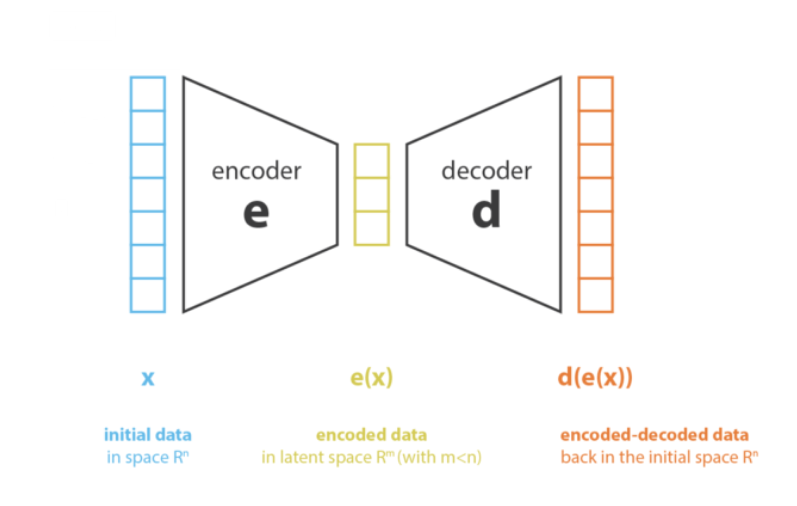
\includegraphics[width=0.90\textwidth]{figs/encoder-decoder.png}
	\caption{Strutture generale di un processo di riduzione della dimensionalità . L'immagine è presa da \cite{Understanding_VAEs}}
	\label{encoder-decoder}
\end{figure}

Il vettore di input $\textbf{x}$ (n-dimensionale) viene compresso dall'encoder $\textbf{e}$ in un vettore $\textbf{e}(\textbf{x})$ di uno spazio m-dimensionale (con m<n), detto $\textit{spazio latente}$; l'encoder, come detto, può agire per selezione o per estrazione. \\
Il decoder $\textbf{d}$ svolge la funzione opposta, ovvero decomprime il vettore $\textbf{e}(\textbf{x})$ in $\textbf{d}(\textbf{e}(\textbf{x}))$ per tornare allo spazio originario n-dimensionale. \\
Nel caso in cui $\textbf{x} = \textbf{d}(\textbf{e}(\textbf{x}))$ (caso ideale) si dice che il processo è un $\textit{lossless encoding}$, ovvero non c'è stata perdita di informazioni nella riduzione della dimensionalità; viceversa, se $\textbf{x} \not= \textbf{d}(\textbf{e}(\textbf{x}))$, si parla di un $\textit{lossy encoding}$, cioè un processo nel quale parte dell'informazione viene persa e non può essere recuperata con la fase di decoding. \\
\newpage
Come conseguenza di ciò che è stato appena illustrato, l'obiettivo di un processo di riduzione della dimensionalità è quello di trovare la coppia encoder-decoder (e,d) fra una famiglia di encoder E e di decoder D, che minimizzi l'informazione persa:
\begin{equation}
(e,d) = \min_{E \times D} \epsilon (\textbf{x},\textbf{d}(\textbf{e}(\textbf{x})))
\end{equation}
dove $\epsilon (\textbf{x},\textbf{d}(\textbf{e}(\textbf{x})))$ è la grandezza attraverso la quale viene  quantificata la quantità di informazione persa nel processo di riduzione. \\ \\
A questo punto è possibile illustrare le varie metodologie di riduzione della dimensionalità, secondo la distinzione già incontrata fra selezione ed estrazione. \\
I metodi di selezione ("$\textit{Feature Selection Methods}$ (FSM)") sono metodi attraverso i quali vengono selezionate le componenti dei vettori di input da tenere e quelle da eliminare perché irrilevanti per le analisi successive. I FSM si includo i $\textit{wrapper methods}$ ed i $\textit{filter methods}$: i primi valutano il modello con varie combinazioni di subset delle variabili originali e selezionano quella con la più alta efficienza, mentre i secondi utilizzano un metodo basato su dei punteggi per valutare eventuali correlazioni fra le variabili di partenza. \\
I metodi di estrazione, invece, si basano fortemente sull'algebra lineare; in particolare vengono utilizzati spesso per la riduzione della dimensionalità i metodi di fattorizzazione delle matrici per cogliere la parte più importante dei dati. \\
Il più comune di questi metodi prende il nome di $\textit{Principal Component Analysis}$ (PCA), del quale verrà presentata brevemente l'idea di base, evitando di addentrarsi troppo nella trattazione matematica che è essenzialmente riconducibile ad un calcolo di autovalori ed autovettori. \\
L'idea del PCA è quella di costruire un numero $\textit{n}_\textit{e}$ di nuove variabili indipendenti che siano combinazione lineare delle $\textit{n}$ variabili di partenza; tale costruzione viene fatta in modo tale che la proiezione delle vecchie variabili sul nuovo sottospazio generato da quelle nuove sia il più possibile vicina ai dati iniziali, dove la vicinanza è da intendere in termini della distanza euclidea. In altre parole con il PCA si ricerca il sottospazio dello spazio dei pattern di partenza per il quale l'errore che viene compiuto nell'approssimazione dei dati tramite proiezioni sia il più piccolo possibile. Si riporta in figura ~\ref{PCA} un'illustrazione di ciò che è stato appena detto.
\\
\begin{figure}[h!]
	\centering
	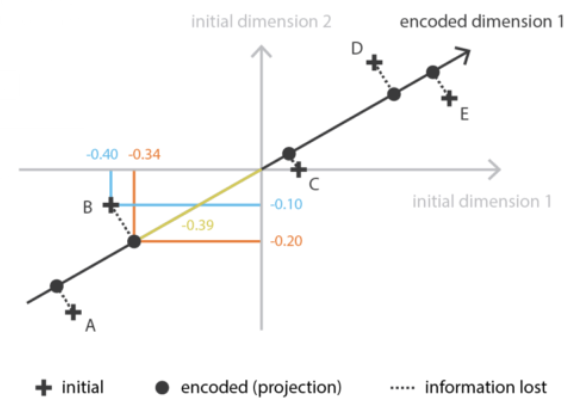
\includegraphics[width=0.57\textwidth]{figs/PCA.png}
	\caption{Illustrazione del processo di PCA nel caso di uno spazio dei pattern iniziali bi-dimensionale (\cite{Understanding_VAEs}).}
	\label{PCA}
\end{figure}

\newpage

\subsection{Autoencoders}
\label{autoencoders}
Gli autoencoders, come ogni altro metodo di riduzione della dimensionalità, sono costituiti da un encoder e da un decoder; tuttavia in questo caso la peculiarità è che sia l'encoder che il decoder sono delle reti neurali, come è possibile vedere in figura ~\ref{autoencoder}. 

\begin{figure}[h!]
	\centering
	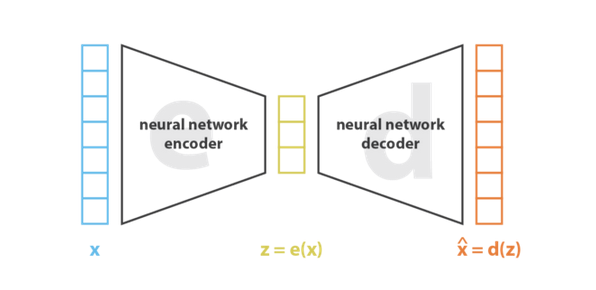
\includegraphics[width=0.70\textwidth]{figs/autoencoder.png}
	\caption{Struttura di un generico autoencoder (\cite{Understanding_VAEs}).}
	\label{autoencoder}
\end{figure}

L'obiettivo è chiaramente quello di individuare la coppia encoder-decoder che ottimizza il processo di ricostruzione degli input e ciò viene fatto attraverso il seguente processo iterativo: si presentano all'encoder i pattern di partenza uno alla volta, subiscono un processo di riduzione della dimensionalità e poi vengono ricostruiti (tornando alla dimensionalità di partenza), viene calcolato l'errore dal confronto fra l'input iniziale e quello ricostruito ed avviene l'aggiornamento dei pesi della rete neurale mediante il meccanismo di backpropagation, già incontrato nella sezione ~\ref{reti neurali}. \\
Intuitivamente l'autoencoder può essere pensato come un collo di bottiglia, attraverso il quale solo una parte dell'informazione riesce a passare oltre e a formare i vettori dello spazio latente.
Facendo riferimento alla figura ~\ref{autoencoder} si osserva che, a partire dai pattern in input \textbf{x}, come primo passo si costruisce lo spazio latente degli $\textbf{z} = e(\textbf{x})$ per poi procedere alla fase di decodifica nella quale si ottengono i pattern ricostruiti $\hat{\textbf{x}} = d(\textbf{z})$; si procede successivamente al calcolo degli errori nel seguente modo:
\begin{equation}
	L = \Vert \textbf{x} - \hat{\textbf{x}} \Vert
\end{equation}
dove L è l'errore di ricostruzione.\\
Una considerazione necessaria circa l'errore, che potrebbe sembrare in contraddizione con quanto detto fino ad ora sul concetto di ottimizzazione, è che si vuole di norma evitare che $\textbf{x} = \hat{\textbf{x}}$, perché questo vuol dire che l'autoencoder ha imparato la funzione identità e, come conseguenza, la struttura dello spazio latente, che è quella interessante per il processo di riduzione della dimensionalità, non porta alcuna informazione interessante; ciò è dovuto al fatto che l'encoder non impara se vi siano variabili più o meno importanti di altre o se esse possano essere compattate in nuove variabili di dimensionalità minore. \\
Per fornire un esempio pratico di ciò che è stato appena affermato, si consideri un insieme di vettori di input N dimensionali; una possibilità è quella di prendere una per una le componenti dei pattern e disporle lungo una retta (spazio latente 1-dimensionale) nella fase di encoding, per poi procedere in maniera inversa nella fase di decodifica. L'errore con questo procedimento sarà nullo ma non si può essere soddisfati essenzialmente per due motivi, ovvero perché lo spazio latente non è interpretabile e sfruttabile e perché in un processo di riduzione della dimensionalità si vuole fare in modo che i dati continuino a conservare una qualche struttura. \\
Una possibilità per evitare il risultato appena illustrato, che è in fin dei conti una sfaccettatura del concetto di overfitting, è di aggiungere alla funzione L un fattore di regolarizzazione che penalizza i risultati per i quali $\textbf{x} = \hat{\textbf{x}}$. \\
Quindi bisogna sempre porre particolare attenzione alla scelta della profondità dell'encoder, ovvero alla sua capacità di riduzione della dimensionalità. \\
Per completezza nella trattazione si osserva che gli autoencoder possono essere sia lineari che non; il primo caso si ottiene quando non si inserisce una funzione di attivazione non lineare e quindi le trasformazioni possono essere rappresentate come matrici, ottenendo un risultato simile a quello del PCA (~\ref{curse_dim}). \\
Il caso di autoencoder non lineari può essere pensato come un passo successivo per quanto riguarda la riduzione della dimensionalità. Infatti, come è stato già detto, il PCA ricerca il miglior iperpiano nello spazio dei pattern originali sul quale questi possano essere proiettati in modo da ridurre la perdita di informazione; dall'altro lato gli autoencoder non lineari non si limitano alla ricerca di iperpiani, ma possono esplorare anche superfici più complesse, come si evince chiaramente dalla figura ~\ref{autoencoder non lineari}.

\begin{figure}[h!]
	\centering
	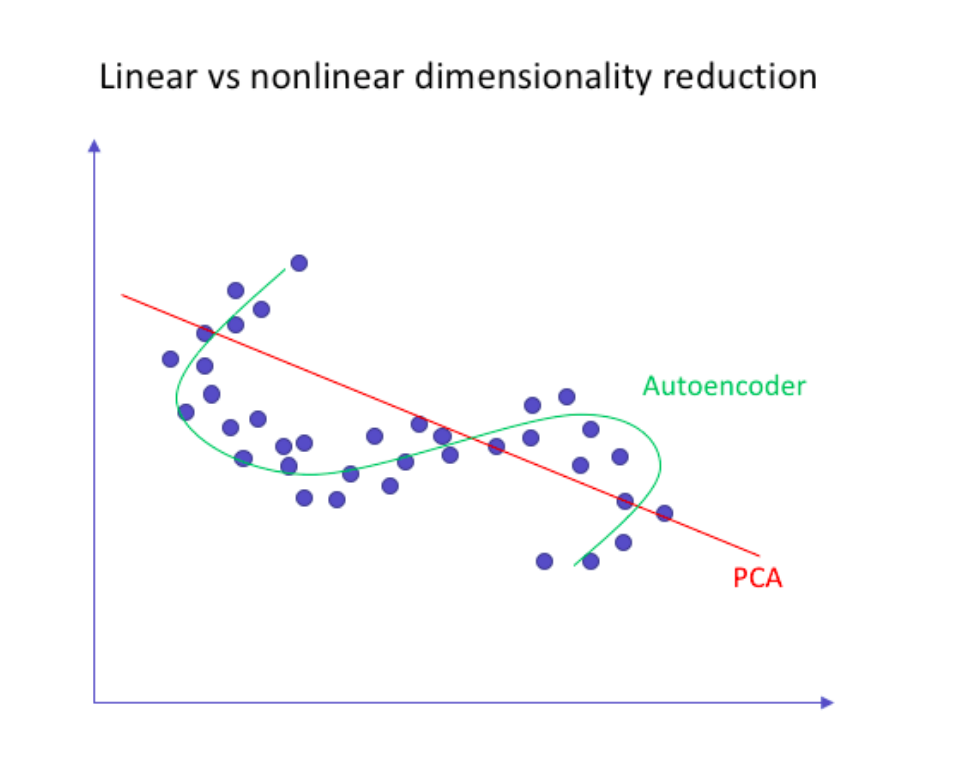
\includegraphics[width=0.70\textwidth]{figs/Autoencoder_non_lineari.png}
	\caption{Differenza fra i metodi lineari (PCA) e gli autoencoder non lineari (\cite{Autoencoders}).}
	\label{autoencode_non_lineari}
\end{figure}




\newpage

\subsection{Variational Autoencoders (VAEs)}
\label{VAEs}

\newpage